% Auto-generated editable source. Edit freely in VS Code.
% Parallel source; the live site is pages/proj-fitness-proxies.html.
\documentclass[11pt]{article}
\usepackage[margin=1in]{geometry}
\usepackage{graphicx}
\usepackage{hyperref}
\usepackage{xcolor}
\definecolor{aidred}{HTML}{A8324A}
\definecolor{aidpink}{HTML}{CF4D87}
\hypersetup{colorlinks=true,linkcolor=aidpink,urlcolor=aidpink,citecolor=aidpink}
\newcommand{\finding}[2]{\par\medskip\noindent{\color{aidred}\textbf{Finding #1.}}~#2\par\medskip}

\title{Gauntlet: Stress-Testing Protein Fitness Proxies}
\author{Saanvi S. Subramanian \\ \small California Institute of Technology}
\date{\small poster, AI for Science @ NeurIPS 2026 \quad\textbullet\quad sole author}
\begin{document}
\maketitle

\begin{abstract}
\noindent A protein fitness proxy is a computable stand-in for a slow wet-lab measurement, and a design campaign ranks thousands of candidates by it and tests the top ones. Gauntlet stress-tests a proxy before anyone ranks designs with it, by asking whether it beats a trivial baseline on measured outcomes, stays useful in the top-ranked region a search actually selects, and resists being driven to pathological inputs. On 504 measured PET-hydrolase variants across 25 studies, an ESM-2 650M zero-shot score ranks activity at a within-study Spearman of 0.01, a substitution matrix is negative, and a plain count of mutations reaches 0.25. A score that cannot beat counting edits is not measuring function on the task it is sold for.
\end{abstract}

\section*{A score that cannot beat counting}
The simplest bar a proxy has to clear is a trivial baseline, and the clearest trivial baseline for a mutant is how many mutations it carries. On PET-hydrolytic activity, a zero-shot ESM-2 650M log-likelihood score ranks variants at a within-study Spearman of 0.01, a substitution matrix scores below zero, a hydropathy feature does better, and a plain mutation count reaches 0.25. The expensive model is the weakest of the four scorers on the property a design campaign would use it for.

\begin{figure}[h]\centering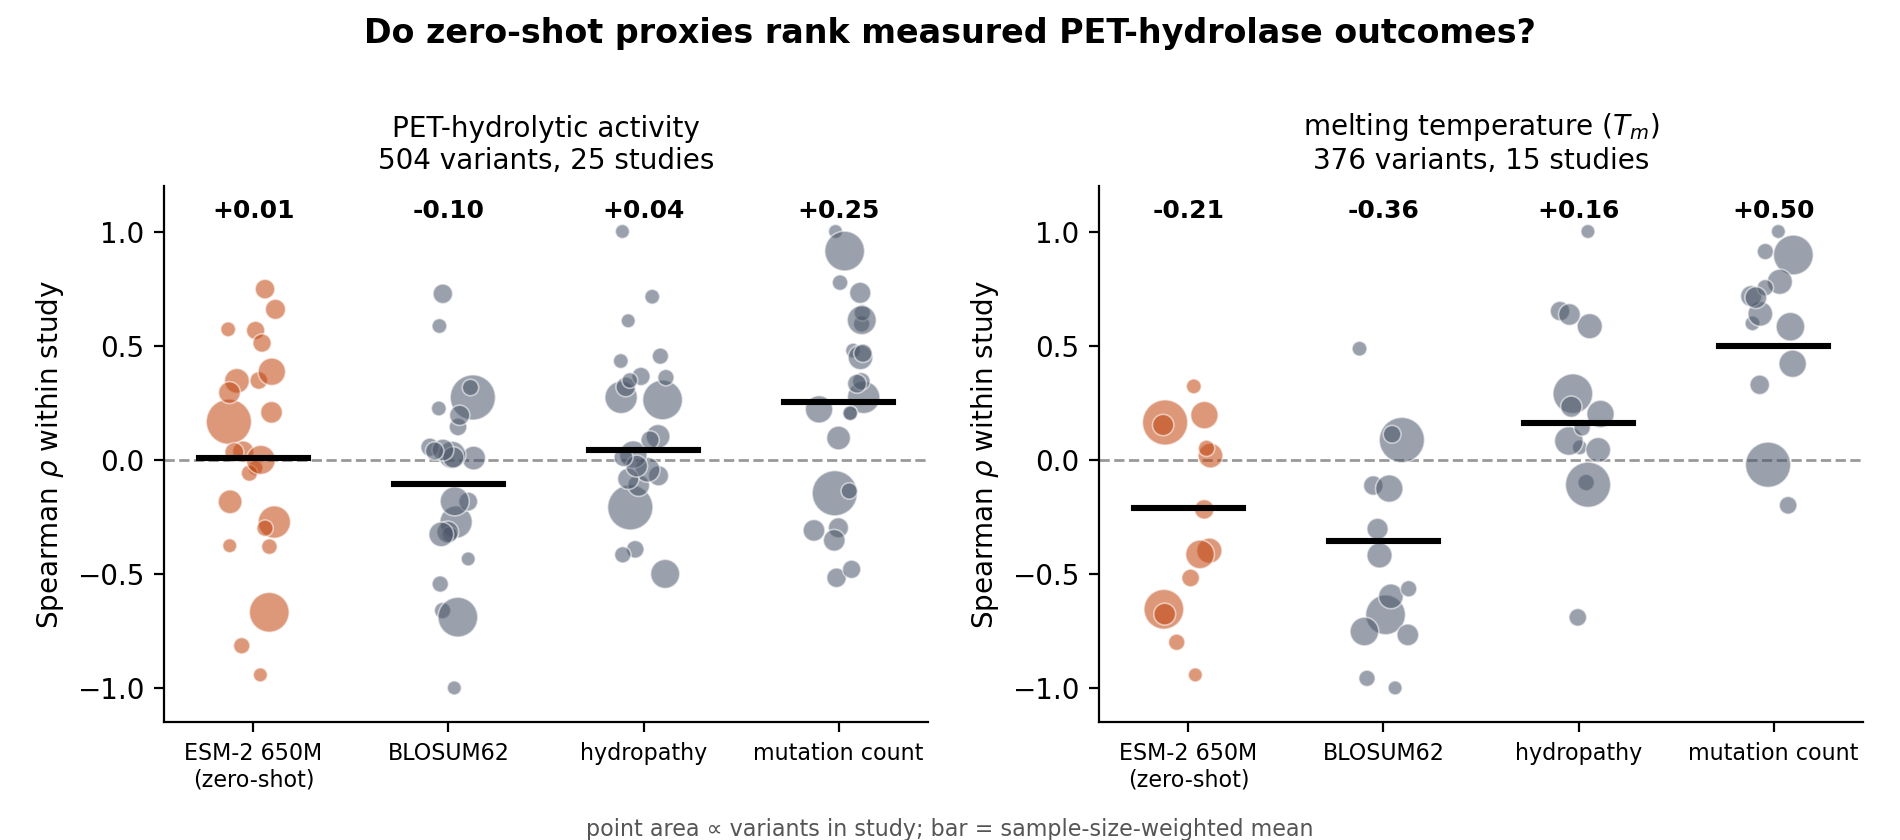
\includegraphics[width=\textwidth]{../../assets/images/projects/eval/gauntlet-proxy-audit.png}
\caption*{\textcolor{aidred}{\textbf{Figure 1. Within-study rank correlation with measured outcomes for four scorers.}} On PET-hydrolytic activity (504 variants, 25 studies) and melting temperature (376 variants, 15 studies). The ESM-2 650M zero-shot score sits near zero on activity, below a hydropathy feature and well below a mutation count at 0.25. The comparison is within study, so it is not confounded by between-study offsets.}\end{figure}

\finding{1}{A zero-shot protein language model ranks measured PETase activity at a within-study Spearman of 0.01, worse than a mutation count at 0.25, so it adds nothing over a trivial baseline on the task it is used for. A proxy that cannot clear counting is not evidence about function, whatever its benchmark correlation elsewhere.}

\paragraph{Why run the audit before the campaign.} The proxy is the score people reach for first when they rank designs without measuring them, and the moment a search starts choosing the candidates it likes best, the proxy is steering the campaign rather than describing it. The three gauntlet checks, beat a trivial baseline, stay useful in the top-ranked tail, and resist an optimizer, are the questions whose answers decide whether the first ranked batch is worth synthesizing. This axis reports the first check; the others are in the broader evaluations program.

\section*{Limitations}
This axis reports one property, PET-hydrolytic activity, with a second on melting temperature, drawn from published measured variants; it is a statement about these assays and these scorers, not a universal ranking of protein models. Zero-shot log-likelihood is one way to score a model, and a supervised or embedding-based readout can do better. The top-tail and reward-hacking checks that complete the gauntlet battery live in the broader evaluations work and are not re-reported here.

\end{document}
